\documentclass[11pt,a4paper]{article}
\usepackage[T1]{fontenc}
\usepackage[utf8]{inputenc}
\usepackage{lmodern,microtype}
\usepackage[margin=.85in]{geometry}
\usepackage{amsmath,amssymb,mathtools}
\usepackage{booktabs,tabularx,array,enumitem,needspace,float}
\usepackage[section]{placeins}
\usepackage{xcolor,tikz,mdframed}
\usetikzlibrary{arrows.meta,positioning,calc}
\usepackage[hidelinks]{hyperref}
\usepackage[nameinlink,noabbrev]{cleveref}
\usepackage{fancyhdr}
\hypersetup{pdftitle={Sync HotStuff, Part 0: Original Protocol},
  pdfsubject={The standard-synchrony baseline for Sync HotStuff RR}}
\setlength{\headheight}{14pt}
\pagestyle{fancy}\fancyhf{}
\lhead{\small Sync HotStuff, Part 0}\rhead{\small Original protocol}
\cfoot{\thepage}
\setlength{\parindent}{0pt}\setlength{\parskip}{4pt}
\setlength{\emergencystretch}{2em}
\setlist{nosep,leftmargin=*}
\newcolumntype{Y}{>{\raggedright\arraybackslash}X}
\definecolor{syncBlue}{HTML}{2563EB}
\definecolor{syncTeal}{HTML}{0F766E}
\newcommand{\QC}{\mathcal C}
\newcommand{\Hash}{\mathsf H}
\newcommand{\rank}{\operatorname{rank}}
\newcommand{\tagg}[1]{\ensuremath{\mathsf{#1}}}
\newcommand{\signed}[2]{\langle #1\rangle_{#2}}
\newcounter{protocol}
\newenvironment{protocol}[2]{\refstepcounter{protocol}\label{#1}
\begin{mdframed}[nobreak=true,linewidth=.6pt,skipabove=8pt,skipbelow=8pt,
innertopmargin=7pt,innerbottommargin=7pt]\small
\textbf{Protocol \theprotocol. #2}\par\smallskip}{\end{mdframed}}
\crefname{protocol}{Protocol}{Protocols}
\Crefname{protocol}{Protocol}{Protocols}
\title{Sync HotStuff, Part 0: Original Protocol\\
  \large Standard Synchrony and the Chained Pipeline}
\author{}\date{13 October 2026}

\begin{document}
\maketitle
\begin{abstract}
This document records the original Sync HotStuff protocol under standard
synchrony, as presented in Section II and Figures 1--2 of Abraham et
al.~\cite{sync}. It supplies the baseline for Part~I's regular leader
rotation and Part~II's sequencer service. We specify blocks, certificates,
the proposal--vote pipeline, local commitment, and lock-based view change.
The pipeline diagrams are adapted from the earlier regional drafts to
the original protocol's replica counts and messages.
\end{abstract}

\section{Scope and model}
\label{sec:scope}
We use the published IEEE S\&P 2020 paper~\cite{sync}, specifically its
\emph{standard-synchrony} protocol. The paper separately extends this
baseline to mobile sluggish faults and optimistic responsiveness in
Sections III--IV. Those extensions are outside Part~0.

There are $n=2f+1$ replicas, at most $f$ of them Byzantine. Messages use
authenticated pairwise channels and transferable digital signatures.
The known delay bound is $\Delta$; actual message delay is
$\delta\leq\Delta$. Correct replicas' messages arrive within that bound.
Clocks run at the same rate, so local waits measure the same elapsed
time. The protocol does not require replicas to execute in lockstep.
For this restatement, delivery includes the block and ancestry needed
to validate the message.

A \emph{view} $v$ has one leader $L_v$, for example replica $v\bmod n$.
That leader keeps proposing until the view is abandoned because of
insufficient progress or leader equivocation. There is no block quota
or scheduled change inside a healthy view.

Safety means that correct replicas never commit different blocks at one
height. A commitment retains the entire ancestor prefix. Liveness means
continued commitment of new blocks; including a particular client
request also needs the leader to receive and eventually select it.

\section{Blocks, certificates, and local state}
\label{sec:objects}
\paragraph{Blocks and conflicts.}
A block has the form
\[
 B_k=(b_k,\Hash(B_{k-1})),
\]
where $b_k$ is a batch of commands. Validation checks both the parent
chain and application validity relative to that chain. We write
$B\preceq B'$ when $B'$ extends $B$, including equality. Blocks conflict
when neither extends the other. Thus conflicting branches can be
detected even when their tips have different heights.

We use a common initial block $B_0$ as a notation convention compatible
with Part~I. The paper instead writes its first block with a null parent.
The initial checkpoint is trusted; later view openings obtain their
current-view certificates through \cref{alg:change}.

\paragraph{Certificates and rank.}
Write $\signed{m}{r}$ for replica $r$'s signature on message $m$.
A quorum certificate $\QC_v(B_k)$ contains $f+1$ matching votes
$\signed{\tagg{VOTE},B_k,v}{r}$ from distinct replicas. Its rank is
\[
 \rank(\QC_v(B_k))=(v,k),
\]
ordered lexicographically, with the view compared first. A certificate
contains at least one correct vote. Two majority quorums need not
intersect in a correct replica; synchrony and the commit wait supply
the additional safety argument.

Certification and commitment are different events. A certificate permits
the leader to propose a child. It does not certify that any replica's
commit timer has expired. The same block may acquire a certificate in a
later view without changing its contents or parent.

\paragraph{Replica state.}
Each replica retains its current view, known signed leader messages,
known certificates, highest-ranked certificate, entry lock, committed
prefix, and running commit timers. A timer belongs to a proposal that
the replica voted for, and starts at that replica's own vote time.
Duplicates do not create another vote or restart a timer. A replica
checks signatures, certificate signers, block validity, and the view
before acting. Forwarding preserves the leader's original signature.
At equal timestamps, process delivered quit or equivocation evidence
before an expiring commit timer.

\section{Steady operation}
\label{sec:steady}
The following box restates Figure~1 of the paper in this notation.
The leader begins with a current-view certificate for the inherited
block, obtained at initialization or through \cref{alg:change}.

\begin{protocol}{alg:steady}{Propose, forward and vote, commit}
\textbf{Current view:} $v$, with leader $L_v$.
\begin{enumerate}[label=\textbf{S\arabic*.},itemsep=4pt]
\item \textbf{Propose (leader).} On obtaining $\QC_v(B_{k-1})$,
construct a valid child $B_k$ and broadcast
\[
 P_k=\signed{\tagg{PROPOSE},B_k,v,\QC_v(B_{k-1})}{L_v}.
\]
The parent certificate must be from the current view.

\item \textbf{Forward and vote (each replica $r$).} On receiving a
valid $P_k$, directly or through a relay, while still in view $v$ and
without detected leader equivocation, forward $P_k$ to all replicas
and broadcast $\signed{\tagg{VOTE},B_k,v}{r}$. At this vote time
$\tau_r(B_k)$, start the block's local $2\Delta$ commit timer.
Matching votes are collected into $\QC_v(B_k)$.

\item \textbf{Commit (each replica $r$, concurrently).} At
$\tau_r(B_k)+2\Delta$, if $r$ has not quit view $v$ or detected leader
equivocation, commit $B_k$ and all its uncommitted ancestors in order.
This wait does not delay voting on later proposals.
\end{enumerate}
As soon as $L_v$ obtains $\QC_v(B_k)$, it repeats S1 for $B_{k+1}$.
It does not wait for $B_k$ to commit.
\end{protocol}

\paragraph{Leader equivocation.}
Two signed \tagg{PROPOSE} or \tagg{NEWVIEW} messages of the same
leader in the same view are evidence if the blocks they identify
conflict. A replica relays the evidence and quits under
\cref{alg:change}. The conflict check concerns the complete branches,
not only two different blocks at the same height.

\section{The chained pipeline}
\label{sec:pipeline}
% Pipeline layouts migrated from formalization/main_v2.tex and its
% versioned successors, with original-protocol notation and replica counts.
\Cref{fig:pipeline} separates the certificate that advances the chain
from the wait that commits each block. \Cref{fig:communication} expands
the same events into proposal delivery and all-to-all forwarding and votes.

\begin{figure}[H]\centering
% Adapted from formalization/figures/v2-major/regional-pipeline.tex.
% Original count-based Sync HotStuff: no stake weights or stream receipts.
% Time is schematic; the overlap illustrates delta < Delta.
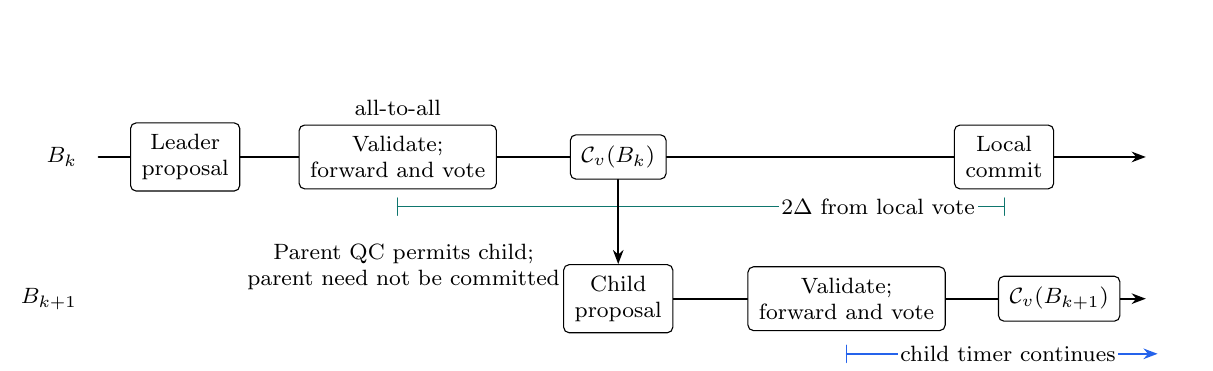
\begin{tikzpicture}[
  x=1cm,y=1cm,font=\footnotesize,line cap=round,line join=round,
  flow/.style={-{Stealth[length=1.8mm]},semithick},
  event/.style={draw,rounded corners=2pt,align=center,fill=white,inner sep=4pt},
  lab/.style={fill=white,inner sep=1pt,align=center}
]
  \path[use as bounding box] (0,-.3) rectangle (14.7,3.7);
  \node[anchor=east] at (.75,2.55) {$B_k$};
  \draw[flow] (.9,2.55) -- (14.2,2.55);
  \node[event] (prop) at (2.0,2.55) {Leader\\proposal};
  \node[event] (vote) at (4.7,2.55) {Validate;\\forward and vote};
  \node[event] (qc) at (7.5,2.55) {$\QC_v(B_k)$};
  \node[event] (commit) at (12.4,2.55) {Local\\commit};
  \node[lab] at (4.7,3.17) {all-to-all};
  \draw[semithick,syncTeal] (4.7,1.92) -- (12.4,1.92);
  \draw[syncTeal] (4.7,1.81) -- (4.7,2.03);
  \draw[syncTeal] (12.4,1.81) -- (12.4,2.03);
  \node[lab] at (10.8,1.92) {$2\Delta$ from local vote};

  \node[anchor=east] at (.75,.75) {$B_{k+1}$};
  \draw[flow] (7.5,.75) -- (14.2,.75);
  \node[event] (child) at (7.5,.75) {Child\\proposal};
  \node[event] (cvote) at (10.4,.75) {Validate;\\forward and vote};
  \node[event] (cqc) at (13.1,.75) {$\QC_v(B_{k+1})$};
  \draw[flow] (qc.south) -- (child.north);
  \node[lab,anchor=east] at (6.8,1.15)
    {Parent QC permits child;\\parent need not be committed};
  \draw[semithick,syncBlue] (10.4,.05) -- (14.0,.05);
  \draw[syncBlue] (10.4,-.06) -- (10.4,.16);
  \draw[flow,syncBlue] (14.0,.05) -- (14.35,.05);
  \node[lab] at (12.45,.05) {child timer continues};
\end{tikzpicture}

\caption{One stable leader pipelines successive blocks in view $v$.
The certificate of $B_k$ permits $B_{k+1}$ before $B_k$ commits.
Each timer starts at the corresponding local vote, not at QC formation.
Time is schematic; the illustrated overlap assumes $\delta<\Delta$.}
\label{fig:pipeline}
\end{figure}

\begin{figure}[H]\centering
% Adapted from the regional communication pipeline and Part I's timer bars.
% Native standard-synchrony messages, n = 3, f = 1, no consumer receipt.
% An honest-leader trace; delta << Delta so timers overlap.
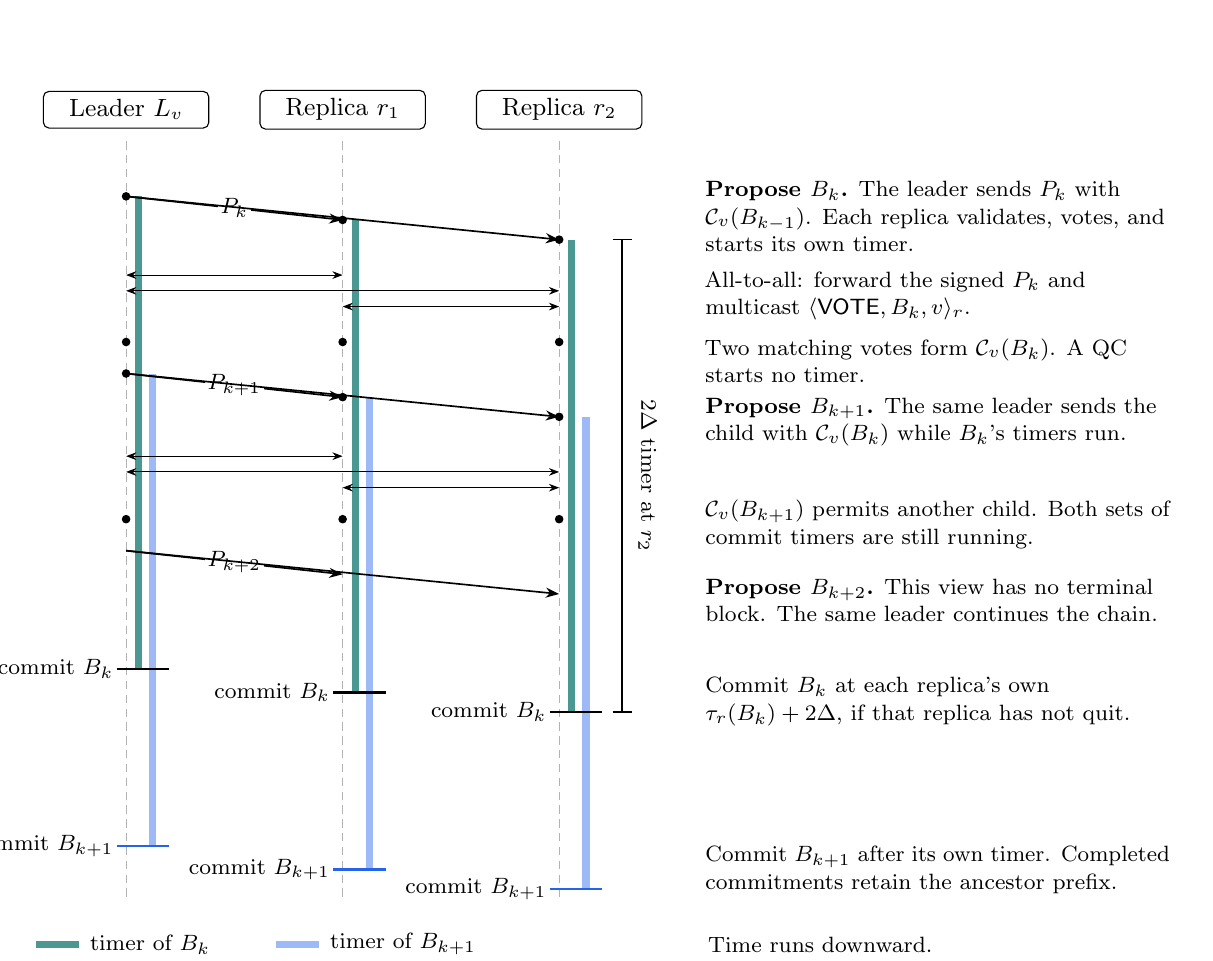
\begin{tikzpicture}[
  x=1cm,y=-1cm,font=\fontsize{9}{10.5}\selectfont,
  party/.style={draw,rounded corners=2pt,fill=white,align=center,
    inner sep=3pt,minimum width=2.1cm},
  lane/.style={draw=black!30,densely dashed},
  msg/.style={-{Stealth[length=1.7mm]},semithick},
  xchg/.style={{Stealth[length=1.3mm]}-{Stealth[length=1.3mm]},thin},
  tag/.style={fill=white,inner sep=1pt,font=\fontsize{8}{9}\selectfont},
  note/.style={anchor=north west,align=flush left,text width=5.9cm,
    inner sep=0pt,font=\fontsize{8.5}{10}\selectfont},
  dot/.style={circle,fill=black,inner sep=1.1pt},
  timerA/.style={line width=2.6pt,draw=syncTeal!75},
  timerB/.style={line width=2.6pt,draw=syncBlue!45}
]
  \def\xL{1.15}\def\xa{3.9}\def\xb{6.65}\def\xn{8.5}
  \path[use as bounding box] (-.1,-.55) rectangle (14.6,10.95);
  \node[party] at (\xL,0) {Leader $L_v$};
  \node[party] at (\xa,0) {Replica $r_1$};
  \node[party] at (\xb,0) {Replica $r_2$};
  \foreach \x in {\xL,\xa,\xb} \draw[lane] (\x,.4)--(\x,10.0);

  % Every complete bar is a local 2 Delta interval (6.0 drawing units).
  \foreach \x/\s in {\xL/1.10,\xa/1.40,\xb/1.65}
    \draw[timerA] (\x+.16,\s)--(\x+.16,\s+6.0);
  \foreach \x/\s in {\xL/3.35,\xa/3.65,\xb/3.90}
    \draw[timerB] (\x+.34,\s)--(\x+.34,\s+6.0);

  \draw[msg] (\xL,1.10)--node[tag,pos=.5] {$P_k$} (\xa,1.40);
  \draw[msg] (\xL,1.10)--(\xb,1.65);
  \foreach \x/\y in {\xL/1.10,\xa/1.40,\xb/1.65}
    \node[dot] at (\x,\y) {};
  \node[note] at (\xn,.9) {\textbf{Propose $B_k$.} The leader sends
    $P_k$ with $\QC_v(B_{k-1})$. Each replica validates, votes,
    and starts its own timer.};

  \draw[xchg] (\xL,2.10)--(\xa,2.10);
  \draw[xchg] (\xL,2.30)--(\xb,2.30);
  \draw[xchg] (\xa,2.50)--(\xb,2.50);
  \node[note] at (\xn,2.05) {All-to-all: forward the signed $P_k$
    and multicast $\signed{\tagg{VOTE},B_k,v}{r}$.};
  \foreach \x in {\xL,\xa,\xb} \node[dot] at (\x,2.95) {};
  \node[note] at (\xn,2.9) {Two matching votes form $\QC_v(B_k)$.
    A QC starts no timer.};

  \draw[msg] (\xL,3.35)--node[tag,pos=.5] {$P_{k+1}$} (\xa,3.65);
  \draw[msg] (\xL,3.35)--(\xb,3.90);
  \foreach \x/\y in {\xL/3.35,\xa/3.65,\xb/3.90}
    \node[dot] at (\x,\y) {};
  \node[note] at (\xn,3.65) {\textbf{Propose $B_{k+1}$.} The same
    leader sends the child with $\QC_v(B_k)$ while $B_k$'s timers run.};
  \draw[xchg] (\xL,4.40)--(\xa,4.40);
  \draw[xchg] (\xL,4.60)--(\xb,4.60);
  \draw[xchg] (\xa,4.80)--(\xb,4.80);
  \foreach \x in {\xL,\xa,\xb} \node[dot] at (\x,5.2) {};
  \node[note] at (\xn,4.95) {$\QC_v(B_{k+1})$ permits another child.
    Both sets of commit timers are still running.};

  \draw[msg] (\xL,5.60)--node[tag,pos=.5] {$P_{k+2}$} (\xa,5.90);
  \draw[msg] (\xL,5.60)--(\xb,6.15);
  \node[note] at (\xn,5.95) {\textbf{Propose $B_{k+2}$.} This view
    has no terminal block. The same leader continues the chain.};

  \foreach \x/\e in {\xL/7.10,\xa/7.40,\xb/7.65} {
    \draw[thick] (\x-.12,\e)--(\x+.55,\e);
    \node[tag,anchor=east] at (\x-.12,\e) {commit $B_k$};
  }
  \node[note] at (\xn,7.20) {Commit $B_k$ at each replica's own
    $\tau_r(B_k)+2\Delta$, if that replica has not quit.};
  \draw[semithick] (7.45,1.65)--(7.45,7.65);
  \draw[semithick] (7.33,1.65)--(7.57,1.65);
  \draw[semithick] (7.33,7.65)--(7.57,7.65);
  \node[tag,rotate=-90] at (7.77,4.65) {$2\Delta$ timer at $r_2$};

  \foreach \x/\e in {\xL/9.35,\xa/9.65,\xb/9.90} {
    \draw[thick,syncBlue] (\x-.12,\e)--(\x+.55,\e);
    \node[tag,anchor=east] at (\x-.12,\e) {commit $B_{k+1}$};
  }
  \node[note] at (\xn,9.35) {Commit $B_{k+1}$ after its own timer.
    Completed commitments retain the ancestor prefix.};
  \draw[timerA] (0,10.6)--(.55,10.6);
  \node[tag,anchor=west] at (.65,10.6) {timer of $B_k$};
  \draw[timerB] (3.05,10.6)--(3.6,10.6);
  \node[tag,anchor=west] at (3.7,10.6) {timer of $B_{k+1}$};
  \node[tag,anchor=west] at (\xn,10.6) {Time runs downward.};
\end{tikzpicture}

\caption{An uninterrupted steady-state example with $n=3$, $f=1$.
The leader is also a voting replica, and a QC needs two votes.
The three pairs of bidirectional arrows denote proposal forwarding and
vote multicast. Each colored bar measures one replica's local timer.
Vertical spacing illustrates $\delta\ll\Delta$, rather than measured
delays.}
\label{fig:communication}
\end{figure}

\paragraph{Timing.}
With an honest leader and a homogeneous actual delay $\delta$, a
proposal reaches replicas in about $\delta$ and their votes return in
another $\delta$. The leader can therefore propose successive blocks
about $2\delta$ apart. A receiving replica commits a block $2\Delta$
after its own vote, or about $\delta+2\Delta$ after the leader's
proposal. These quantities measure different events. A conservative
$\Delta$ increases the commitment wait while the proposal/QC chain can
continue at actual network speed.

\section{View change and safe inheritance}
\label{sec:change}
The following box restates Figure~2 of the paper. Let $e_r(v)$ be
replica $r$'s local entry time to view $v$. Let $N_r(v)$ count distinct
fresh proposals that triggered its steady-state votes in that view;
the opening vote for an inherited block is separate.

\begin{protocol}{alg:change}{Blame, quit, status, new view, first vote}
Let $L=L_v$ and $L'=L_{v+1}$.
\begin{enumerate}[label=\textbf{V\arabic*.},itemsep=4pt]
\item \textbf{Blame and quit.} For every integer $p\geq1$, at
$e_r(v)+(2p+4)\Delta$, if $N_r(v)<p$, broadcast
$\signed{\tagg{BLAME},v}{r}$.
Quit upon receiving either $f+1$ distinct BLAME signatures for $v$
or a pair of leader-signed messages proving equivocation. Broadcast
that proof. Stop voting in $v$ and cancel all unfinished commit
timers of $v$; retain completed commitments.

\item \textbf{Status and entry.} Wait $\Delta$ from the local quit
time, continuing to receive old votes and certificates. Choose a
highest-ranked known certificate $Q_r=\QC_{v_r}(B_{k_r})$ from the
departing or earlier views. Lock on $Q_r$, report it to $L'$ in a
signed STATUS message, and enter view $v+1$.

\item \textbf{New-view announcement (leader $L'$).} Wait $2\Delta$
from $L'$'s own entry to $v+1$. Choose a highest-ranked known
earlier-view certificate $Q^*=\QC_{v^*}(B_{k^*})$, including those
reported in STATUS, and broadcast
\[
 \signed{\tagg{NEWVIEW},v+1,Q^*}{L'}.
\]

\item \textbf{First vote (each replica $r$).} While in view $v+1$,
on receiving a valid NEWVIEW, if no leader equivocation is known and
$\rank(Q^*)\geq\rank(Q_r)$, forward it and broadcast
$\signed{\tagg{VOTE},B_{k^*},v+1}{r}$.
This vote re-certifies the unchanged inherited block. It starts no
commit timer. Once $L'$ obtains $\QC_{v+1}(B_{k^*})$, it proposes
a fresh child under \cref{alg:steady}.
\end{enumerate}
\end{protocol}

\paragraph{The two waits.}
Relaying a quit proof makes correct replicas quit within $\Delta$ of
one another. Their additional $\Delta$ wait allows old votes to form
certificates before each replica fixes its next entry lock. The new
leader's $2\Delta$ wait covers entry skew and STATUS delivery, so a
correct leader learns every correct entry lock before selecting the
new-view block. The fresh child carries a \emph{new-view} certificate
for the inherited block; an old-view QC alone does not resume the
steady-state pipeline.

\section{Why commitment survives recovery}
\label{sec:safety}
Section II-C of the paper supplies the correctness arguments. A correct
vote at time $s$ forwards the proposal to all correct replicas by
$s+\Delta$. Any earlier correct vote on a conflicting proposal would
relay the conflict back by $s+2\Delta$ and prevent commitment.
After detecting a conflict, correct replicas quit.

If the timer survives, the paper shows that the block becomes certified
and every correct replica's next entry lock ranks at least as high as
its certificate. The lock test and current-view parent QCs then protect
the committed prefix in later views. Some replicas may quit before
their own timers expire; recovery still preserves another replica's
completed commitment.

For progress, the blame deadlines end stalled views. Round-robin
selection eventually supplies a correct leader, whose NEWVIEW meets
all correct entry locks and whose proposals sustain the pipeline.
Part~I separately analyzes regular rotation.

\begin{figure}[H]\centering
% Original Sync HotStuff, Figure 2, in the notation of Part 0.
% The replica and leader lanes denote roles within the same fixed committee.
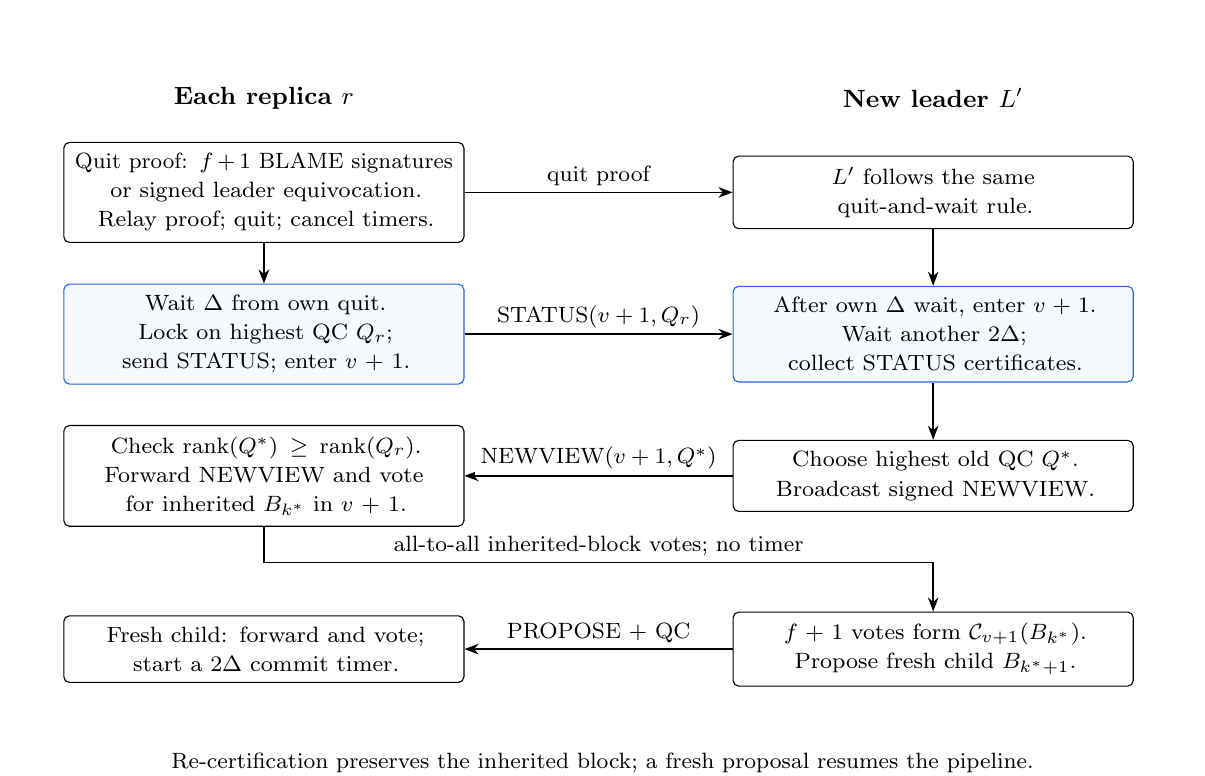
\begin{tikzpicture}[
  x=1cm,y=-1cm,font=\fontsize{8.5}{10.5}\selectfont,
  box/.style={draw,rounded corners=2pt,fill=white,align=center,
    inner sep=4pt,text width=4.8cm},
  wait/.style={box,draw=syncBlue,fill=syncBlue!4},
  flow/.style={-{Stealth[length=1.8mm]},semithick},
  lab/.style={fill=white,inner sep=2pt,align=center,
    font=\fontsize{8.5}{10.5}\selectfont}
]
  \path[use as bounding box] (0,-.4) rectangle (14.6,8.75);
  \node[font=\small\bfseries] at (3.0,0) {Each replica $r$};
  \node[font=\small\bfseries] at (11.5,0) {New leader $L'$};
  \node[box] (quit) at (3.0,1.2)
    {Quit proof: $f+1$ BLAME signatures\\or signed leader equivocation.\\
     Relay proof; quit; cancel timers.};
  \node[box] (lquit) at (11.5,1.2)
    {$L'$ follows the same\\quit-and-wait rule.};
  \draw[flow] (quit.east)--node[lab,above] {quit proof} (lquit.west);
  \node[wait] (status) at (3.0,3.0)
    {Wait $\Delta$ from own quit.\\Lock on highest QC $Q_r$;\\
     send STATUS; enter $v+1$.};
  \node[wait] (entry) at (11.5,3.0)
    {After own $\Delta$ wait, enter $v+1$.\\
     Wait another $2\Delta$;\\collect STATUS certificates.};
  \draw[flow] (quit.south)--(status.north);
  \draw[flow] (lquit.south)--(entry.north);
  \draw[flow] (status.east)--node[lab,above] {STATUS$(v+1,Q_r)$} (entry.west);
  \node[box] (first) at (3.0,4.8)
    {Check $\rank(Q^*)\geq\rank(Q_r)$.\\Forward NEWVIEW and vote\\
     for inherited $B_{k^*}$ in $v+1$.};
  \node[box] (newview) at (11.5,4.8)
    {Choose highest old QC $Q^*$.\\
     Broadcast signed NEWVIEW.};
  \draw[flow] (entry.south)--(newview.north);
  \draw[flow] (newview.west)--node[lab,above] {NEWVIEW$(v+1,Q^*)$} (first.east);
  \node[box] (fresh) at (3.0,7.0)
    {Fresh child: forward and vote;\\start a $2\Delta$ commit timer.};
  \node[box] (recert) at (11.5,7.0)
    {$f+1$ votes form $\QC_{v+1}(B_{k^*})$.\\
     Propose fresh child $B_{k^*+1}$.};
  \draw[flow] (first.south)--(3.0,5.9)--
    node[lab,above] {all-to-all inherited-block votes; no timer}
    (11.5,5.9)--(recert.north);
  \draw[flow] (recert.west)--node[lab,above] {PROPOSE + QC} (fresh.east);
  \node[lab] at (7.3,8.45)
    {Re-certification preserves the inherited block; a fresh proposal resumes the pipeline.};
\end{tikzpicture}

\caption{Recovery after a quit proof. The waits start at local events:
each replica's quit, then the new leader's entry. The inherited block
is re-certified before a fresh child starts a commit timer. Arrows
show representative communication; spacing is schematic.}
\label{fig:change}
\end{figure}

\section{From Part 0 to Part I}
\label{sec:rr}
Part~I~\cite{part1} keeps the forwarding, voting, $2\Delta$ timer,
and lock-based recovery mechanisms. It adds a generation/term pair
$(g,t)$, a fixed number of fresh blocks per term, and a terminal-QC
transition to the next leader. Ordinary term changes preserve timers;
a generation quit cancels them. In the original protocol recorded
here, changing the leader always invokes view change and cancels
unfinished timers of the departing view.

\begin{thebibliography}{9}
\bibitem{sync}
I. Abraham, D. Malkhi, K. Nayak, L. Ren, and M. Yin.
\emph{Sync HotStuff: Simple and Practical Synchronous State Machine Replication}.
IEEE Symposium on Security and Privacy, 2020, pp. 106--118.
Section II, Figures 1--2.
\href{https://conferences.computer.org/sp/pdfs/sp/2020/349700a106.pdf}{Published paper}.
\bibitem{part1}
Sync HotStuff RR, Part I: Core Protocol. Design document, 13 October 2026.
\end{thebibliography}
\end{document}
